\documentclass[12pt,a4paper]{article}
\usepackage{amsmath,amssymb}
\usepackage{graphicx}
\usepackage{listings}
\usepackage{textcomp}
\usepackage{accsupp}
\usepackage{xcolor}
\usepackage{geometry}
\usepackage{subcaption}
\geometry{margin=2.5cm}

% --- تنظیمات نمایش کدها (Listings) ---
\lstset{
    basicstyle=\small\ttfamily,
    backgroundcolor=\color{gray!10},
    frame=single,
    breaklines=true,
    breakatwhitespace=true,
    keywordstyle=\color{blue}\bfseries,
    commentstyle=\color{green!60!black},
    stringstyle=\color{purple},
    showstringspaces=false,
    upquote=true,
    columns=fullflexible,
    keepspaces=true
}

% تعریف زبان YAML برای بستهٔ listings
\lstdefinelanguage{yaml}{
    sensitive=false,
    comment=[l]{\#},
    morestring=[b]',
    morestring=[b]",
    keywords={true,false,null,yes,no,on,off},
    keywordstyle=\color{blue}\bfseries
}

% لایهٔ ActualText باعث می‌شود متن اصلی کد، مستقل از شکست ظاهری خطوط،
% به‌صورت دقیق از PDF انتخاب و کپی شود.

% --- تنظیمات هایپرلینک ---
\usepackage{hyperref}
\hypersetup{
    colorlinks=true,
    linkcolor=blue,
    urlcolor=cyan
}

% --- تنظیمات زی‌پرشین (باید آخرین پکیج لود شود) ---
\usepackage{xepersian}

% تنظیم فونت‌ها
\settextfont{Amiri}
\setlatintextfont{Noto Sans}

\title{\textbf{گزارش جامع پیاده‌سازی، رفع چالش‌ها و راه‌اندازی داشبورد سیستم حسگری راداری وای‌فای (ISAC) با پلتفرم ESPectre}}
\author{امیرعلی یزدانی}
\date{\today}

\begin{document}

\maketitle
\tableofcontents
\newpage

\section{مقدمه و ساختار کلی پروژه}
پلتفرم \lr{ESPectre} یک فریم‌ورک سبک و بی‌درنگ برای استخراج اطلاعات وضعیت کانال (\lr{Channel State Information - CSI}) امواج وای‌فای بر بستر چیپ‌های خانواده \lr{ESP32} است. در این فرآیند، استخراج اطلاعات فاز و دامنه ساب‌کریرها جهت پایش حضور و شدت تلاطم محیط با استفاده از برد \lr{ESP32-S3 (N16R8)} صورت پذیرفته و خروجی‌ها در داشبورد گرافیکی \lr{Home Assistant} یکپارچه‌سازی شده‌اند.

\section{معماری ساختاری ESPHome و عدم نیاز به کدنویسی مستقیم C++}
برخلاف پروژه‌های سنتی امبدد، در این فریم‌ورک هیچ نیازی به کدنویسی دستی \lr{C++} نیست؛ پلتفرم \lr{ESPHome} به‌عنوان یک تولیدکننده هوشمند کد (\lr{Code-Generator}) عمل می‌کند:
\begin{enumerate}
    \item متغیرها و ماژول‌ها در فایل‌های مانیفست متنی با فرمت \lr{YAML} تعریف می‌شوند.
    \item موتور \lr{ESPHome} فایل‌های متنی را خوانده و کدهای بهینه‌شده \lr{C++} متناسب با معماری \lr{ESP-IDF} را تولید می‌کند.
    \item بیلدسیستم \lr{Ninja/CMake} کدها را کامپایل کرده و فایل‌های فریم‌ورک باینری را ایجاد می‌نماید.
\end{enumerate}
این سازوکار دارای کمترین سربار حافظه (\lr{Zero-Bloat}) بوده و هسته \lr{ESPectre} تنها حدود \textbf{۷۰ کیلوبایت} از فلش و کمتر از \textbf{۱۰۰ بایت} از رم را مصرف می‌کند.

\section{مراحل آماده‌سازی و نصب بسته‌های پایه}

\subsection{ایجاد محیط مجازی و نصب ابزار ESPHome}
\begin{latin}
\BeginAccSupp{method=hex,ActualText={6364207e2f4465736b746f702f416d6972616c692f5769666953656e73696e672f65737065637472652f65737065637472650a707974686f6e33202d6d2076656e762076656e760a736f757263652076656e762f62696e2f61637469766174650a707974686f6e33202d6d2070697020696e7374616c6c20657370686f6d650a}}
\begin{lstlisting}[language=bash]
cd ~/Desktop/Amirali/WifiSensing/espectre/espectre
python3 -m venv venv
source venv/bin/activate
python3 -m pip install esphome
\end{lstlisting}
\EndAccSupp{}
\end{latin}

\subsection{تعریف متغیرهای دسترسی شبکه (secrets.yaml)}
برای مدیریت امن مشخصات شبکه، فایل \lr{secrets.yaml} در مسیر نمونه‌ها ایجاد گردید:
\begin{latin}
\BeginAccSupp{method=hex,ActualText={636174203e206578616d706c65732f736563726574732e79616d6c203c3c2027454f46270a776966695f737369643a20225368617269662d57694669220a776966695f70617373776f72643a2022220a454f460a}}
\begin{lstlisting}[language=bash]
cat > examples/secrets.yaml << 'EOF'
wifi_ssid: "Sharif-WiFi"
wifi_password: ""
EOF
\end{lstlisting}
\EndAccSupp{}
\end{latin}

\section{اصلاح فایل‌های پیکربندی سخت‌افزاری و نرم‌افزاری}
جهت تطابق فریمور با برد \lr{ESP32-S3-N16R8} (دارای ۱۶ مگابایت فلش و ۸ مگابایت \lr{Octal PSRAM})، اصلاحات ساختاری زیر اعمال شد:

\subsection{اصلاح فایل espectre-s3.yaml}
فعال‌سازی حافظه \lr{Octal PSRAM} و هدایت لاگ‌ها به \lr{USB-JTAG}:
\begin{latin}
\BeginAccSupp{method=hex,ActualText={65737033323a0a202076617269616e743a20455350333253330a20206370755f6672657175656e63793a203234304d487a0a2020626f6172643a2065737033322d73332d6465766b6974632d310a20206672616d65776f726b3a0a20202020747970653a206573702d6964660a2020202076657273696f6e3a20352e352e310a2020202073646b636f6e6669675f6f7074696f6e733a0a202020202020434f4e4649475f4553505f44454641554c545f4350555f465245515f4d485a3a2022323430220a202020202020434f4e4649475f53504952414d3a202279220a202020202020434f4e4649475f53504952414d5f4d4f44455f4f43543a202279220a202020202020434f4e4649475f53504952414d5f545950455f4155544f3a202279220a202020202020434f4e4649475f53504952414d5f53504545445f38304d3a202279220a202020202020434f4e4649475f53504952414d5f424f4f545f494e49543a202279220a202020202020434f4e4649475f4553505f434f4e534f4c455f5553425f53455249414c5f4a5441473a202279220a0a707372616d3a0a20206d6f64653a206f6374616c0a202073706565643a2038304d487a0a}}
\begin{lstlisting}[language=yaml]
esp32:
  variant: ESP32S3
  cpu_frequency: 240MHz
  board: esp32-s3-devkitc-1
  framework:
    type: esp-idf
    version: 5.5.1
    sdkconfig_options:
      CONFIG_ESP_DEFAULT_CPU_FREQ_MHZ: "240"
      CONFIG_SPIRAM: "y"
      CONFIG_SPIRAM_MODE_OCT: "y"
      CONFIG_SPIRAM_TYPE_AUTO: "y"
      CONFIG_SPIRAM_SPEED_80M: "y"
      CONFIG_SPIRAM_BOOT_INIT: "y"
      CONFIG_ESP_CONSOLE_USB_SERIAL_JTAG: "y"

psram:
  mode: octal
  speed: 80MHz
\end{lstlisting}
\EndAccSupp{}
\end{latin}

\subsection{اصلاح فایل espectre-s3-dev.yaml}
تنظیم لاگر سخت‌افزاری بر روی کنسول \lr{USB\_SERIAL\_JTAG}:
\begin{latin}
\BeginAccSupp{method=hex,ActualText={6c6f676765723a0a20206c6576656c3a2044454255470a202068617264776172655f756172743a205553425f53455249414c5f4a5441470a20206c6f67733a0a2020202073656e736f723a20494e464f0a2020202062696e6172795f73656e736f723a20494e464f0a}}
\begin{lstlisting}[language=yaml]
logger:
  level: DEBUG
  hardware_uart: USB_SERIAL_JTAG
  logs:
    sensor: INFO
    binary_sensor: INFO
\end{lstlisting}
\EndAccSupp{}
\end{latin}

\section{دستورات پاک‌سازی، کامپایل و مانیتورینگ سریال}

\subsection{پاک‌سازی کامل حافظه فلش}
\begin{latin}
\BeginAccSupp{method=hex,ActualText={736f757263652076656e762f62696e2f61637469766174650a657370746f6f6c2e70792065726173655f666c6173680a}}
\begin{lstlisting}[language=bash]
source venv/bin/activate
esptool.py erase_flash
\end{lstlisting}
\EndAccSupp{}
\end{latin}

\subsection{کامپایل و فلش فریم‌ورک}
\begin{latin}
\BeginAccSupp{method=hex,ActualText={657370686f6d652072756e206578616d706c65732f65737065637472652d73332d6465762e79616d6c0a}}
\begin{lstlisting}[language=bash]
esphome run examples/espectre-s3-dev.yaml
\end{lstlisting}
\EndAccSupp{}
\end{latin}
\textit{در منوی انتخاب پورت، گزینه متناظر با درگاه بومی \lr{/dev/ttyACM0} (عدد ۱) انتخاب شد.}

\subsection{مشاهده لاگ‌های بی‌درنگ}
\begin{latin}
\BeginAccSupp{method=hex,ActualText={657370686f6d65206c6f6773206578616d706c65732f65737065637472652d73332d6465762e79616d6c0a}}
\begin{lstlisting}[language=bash]
esphome logs examples/espectre-s3-dev.yaml
\end{lstlisting}
\EndAccSupp{}
\end{latin}

\section{راه‌اندازی Docker و استقرار سرور \lr{Home Assistant}}

\subsection{تنظیم آینه‌های رجیستری داکر \lr{(Docker Daemon Mirror)}}
به‌دلیل محدودیت‌های دسترسی به رجیستری‌های رسمی، آدرس‌های آینه داخلی درون فایل پیکربندی داکر تنظیم شدند:
\begin{latin}
\BeginAccSupp{method=hex,ActualText={7375646f206d6b646972202d70202f6574632f646f636b65720a7375646f20746565202f6574632f646f636b65722f6461656d6f6e2e6a736f6e203c3c2027454f46270a7b0a20202272656769737472792d6d6972726f7273223a205b0a202020202268747470733a2f2f646f636b65722e617276616e636c6f75642e6972222c0a202020202268747470733a2f2f72656769737472792e646f636b65722e6972220a20205d0a7d0a454f460a7375646f2073797374656d63746c206461656d6f6e2d72656c6f61640a7375646f2073797374656d63746c207265737461727420646f636b65720a}}
\begin{lstlisting}[language=bash]
sudo mkdir -p /etc/docker
sudo tee /etc/docker/daemon.json << 'EOF'
{
  "registry-mirrors": [
    "https://docker.arvancloud.ir",
    "https://registry.docker.ir"
  ]
}
EOF
sudo systemctl daemon-reload
sudo systemctl restart docker
\end{lstlisting}
\EndAccSupp{}
\end{latin}

\subsection{اجرای کانتینر \lr{Home Assistant} با دسترسی به شبکه سیستم}
به‌دلیل تفاوت درگاه شبکه کابل \lr{LAN} سیستم و وای‌فای برد، کانتینر در حالت \lr{--net=host} مستقر گردید تا ارتباطات لایه شبکه محلی مسدود نگردد:
\begin{latin}
\BeginAccSupp{method=hex,ActualText={646f636b65722072756e202d64202d2d6e616d6520686f6d65617373697374616e74202d2d70726976696c65676564202d2d726573746172743d756e6c6573732d73746f70706564202d2d6e65743d686f7374202d6520545a3d417369612f54656872616e202d76207e2f686f6d65617373697374616e745f636f6e6669673a2f636f6e66696720676863722e696f2f686f6d652d617373697374616e742f686f6d652d617373697374616e743a737461626c650a}}
\begin{lstlisting}[language=bash]
docker run -d --name homeassistant --privileged --restart=unless-stopped --net=host -e TZ=Asia/Tehran -v ~/homeassistant_config:/config ghcr.io/home-assistant/home-assistant:stable
\end{lstlisting}
\EndAccSupp{}
\end{latin}

\subsection{پیکربندی گره در پنل تحت وب \lr{Home Assistant} و مدیریت تغییر \lr{IP}}
\begin{enumerate}
    \item ورود به پنل از طریق مرورگر با آدرس \url{http://localhost:8123}.
    \item ورود به مسیر: \lr{Settings} $\rightarrow$ \lr{Devices \& Services} $\rightarrow$ \lr{Add Integration}.
    \item انتخاب ماژول \lr{ESPHome} و وارد کردن دستی آدرس آی‌پی برد (به‌عنوان مثال: \lr{172.27.4.45}) روی پورت پیش‌فرض \textbf{۶۰۵۳}.
\end{enumerate}

\paragraph{مدیریت تغییر آدرس IP دینامیک \lr{(DHCP Re-assignment)}:}
به‌دلیل استفاده از پروتکل \lr{DHCP} در روترها و شبکه‌های محلی، ممکن است پس از هر بار خاموش/روشن شدن برد یا روتر، آدرس \lr{IP} اختصاص‌یافته تغییر کرده و در نتیجه موجودیت‌ها و سنسورها در داشبورد \lr{Home Assistant} در وضعیت ناموجود (\lr{Unavailable}) قرار گیرند. برای رفع این مشکل، مراحل زیر دنبال می‌شود:
\begin{itemize}
    \item \textbf{استخراج آدرس IP جدید:} ابتدا از طریق اتصال کابل \lr{USB} و اجرای دستور زیر، لاگ‌های زنده برد خوانده شده و آدرس جدید در خطوط مربوط به اتصال وای‌فای (مقابل عبارت \lr{\lstinline[basicstyle=\latinfont\ttfamily]|WiFi Connected! IP Address:|)} استخراج می‌گردد:
    \begin{latin}
    \BeginAccSupp{method=hex,ActualText={657370686f6d65206c6f6773206578616d706c65732f65737065637472652d73332d6465762e79616d6c0a202020200a}}
\begin{lstlisting}[language=bash]
esphome logs examples/espectre-s3-dev.yaml
    \end{lstlisting}
\EndAccSupp{}
    \end{latin}
    \item \textbf{پیکربندی مجدد در \lr{Home Assistant}:} بدون نیاز به حذف موجودیت‌ها یا ساخت داشبورد مجدد، در پنل \lr{Home Assistant} به مسیر \lr{Settings} $\rightarrow$ \lr{Devices \& Services} رفته، بر روی کارت مربوط به \lr{ESPHome} و منوی سه‌نقطه گره کلیک کرده و گزینه \textbf{\lr{Reconfigure}} انتخاب می‌شود. با وارد کردن آدرس \lr{IP} جدید و تایید آن، تمام سنسورها و نمودارهای داشبورد بلافاصله به وضعیت فعال (\lr{Active}) بازمی‌گردند.
\end{itemize}

\subsection{ایجاد داشبورد گرافیکی }
پس از ایجاد یک داشبورد جدید، ویرایشگر ساختار خام (\lr{Raw configuration editor}) باز شده و محتویات فایل آماده \lr{examples/home-assistant-dashboard-dev.yaml} درون آن بارگذاری شد تا گیج‌های شدت حرکت، وضعیت آشکارساز و نمودارهای سابقه ۲۴ ساعته فعال گردند.

\paragraph{هشدار مهم در خصوص درگاه اتصال برد \lr{(Hardware Port Warning)}:}
بردهای توسعه \lr{ESP32-S3} معمولاً دارای دو درگاه فیزیکی \lr{Type-C} مجزا هستند. برای فلش، مانیتورینگ زنده سریال و ارتباط مستقیم با کنترلر داخلی \lr{USB-JTAG (ttyACM0)}، کابل \lr{USB} باید \textbf{حتماً به درگاه سمت چپ} برد متصل گردد؛ در غیر این صورت فریم‌ورک شناسایی نشده و ارسال دستورات فلش با خطا مواجه خواهد شد.

\section{تحلیل الگوریتم‌های آشکارسازی: MVS در برابر ML}

\subsection{الگوریتم واریانس متحرک فضایی (MVS)}
این روش آماری، با تحلیل تغییرات تلاطم میدان امواج نسبت به حالت سکون عمل می‌کند:
$$\text{Var}(s) = \frac{1}{N}\sum_{i=1}^N (x_i - \mu)^2$$
در ۱۳ ثانیه اول پس از راه‌اندازی، سیستم در حالت سکون دو فاز \lr{Gain Lock} و کالیبراسیون باند بهینه (\lr{NBVI}) را اجرا کرده و ۱۲ ساب‌کریر با بالاترین سیگنال به نویز را انتخاب می‌نماید.

\subsection{الگوریتم یادگیری ماشین (ML)}
این روش از یک شبکه عصبی پرسپترون چندلایه تعبیه‌شده (\lr{MLP}) با ساختار $9 \rightarrow 32 \rightarrow 16 \rightarrow 1$ بهره می‌برد. زمان راه‌اندازی آن کمتر از \textbf{۳ ثانیه} بوده و به کالیبراسیون نیازی ندارد، اما از ساب‌کریرهای ثابت از پیش‌تعیین‌شده استفاده می‌کند. با تغییر پارامتر \lstinline[basicstyle=\latinfont\ttfamily]|detection_algorithm: ml| در فایل کانفیگ و فلش مجدد، سیستم به حالت عصبی منتقل می‌شود.

\section{مفهوم ISAC و تفاوت بنیادین با پلتفرم RuView}
مفهوم \textbf{مخابرات مجتمع و حسگری (\lr{ISAC})} به بهره‌گیری هم‌زمان از سیگنال‌های ارتباطی استاندارد جهت حسگری محیطی اطلاق می‌گردد:
\begin{itemize}
    \item \textbf{پلتفرم RuView:} داده‌های خام حسگری را در ساختار مش چندنوده (\lr{Multi-Static}) بسته‌بندی کرده و برای تجمیع به یک سرور اختصاصی خارحی (\lr{Rust Server}) مخابره می‌کند.
    \item \textbf{پلتفرم ESPectre:} مفهوم \lr{ISAC} به‌صورت متمرکز درون گره پیاده شده است؛ تراشه با ارسال ترافیک استاندارد شبکه (\lr{Ping/DNS})، اطلاعات \lr{CSI} امواج برگشتی را هم‌زمان استخراج و پردازش‌های آماری/عصبی را بدون نیاز به سرور محاسباتی خارجی در همان لبه سخت‌افزار اجرا می‌نماید.
\end{itemize}

\section{خروجی نهایی و داشبورد پایش}
پس از انجام موفقیت‌آمیز مراحل، داشبورد تحلیلی در بستر \lr{Home Assistant} مستقر گردید که وضعیت بی‌درنگ تلاطم امواج، نمرات حرکت و سوابق حسگری را مصورسازی می‌نماید:

\begin{figure}[htbp]
    \centering
    % تصویر داشبورد را در مسیر مربوطه قرار داده و نام آن را با Dashboard.png جایگزین نمایید
    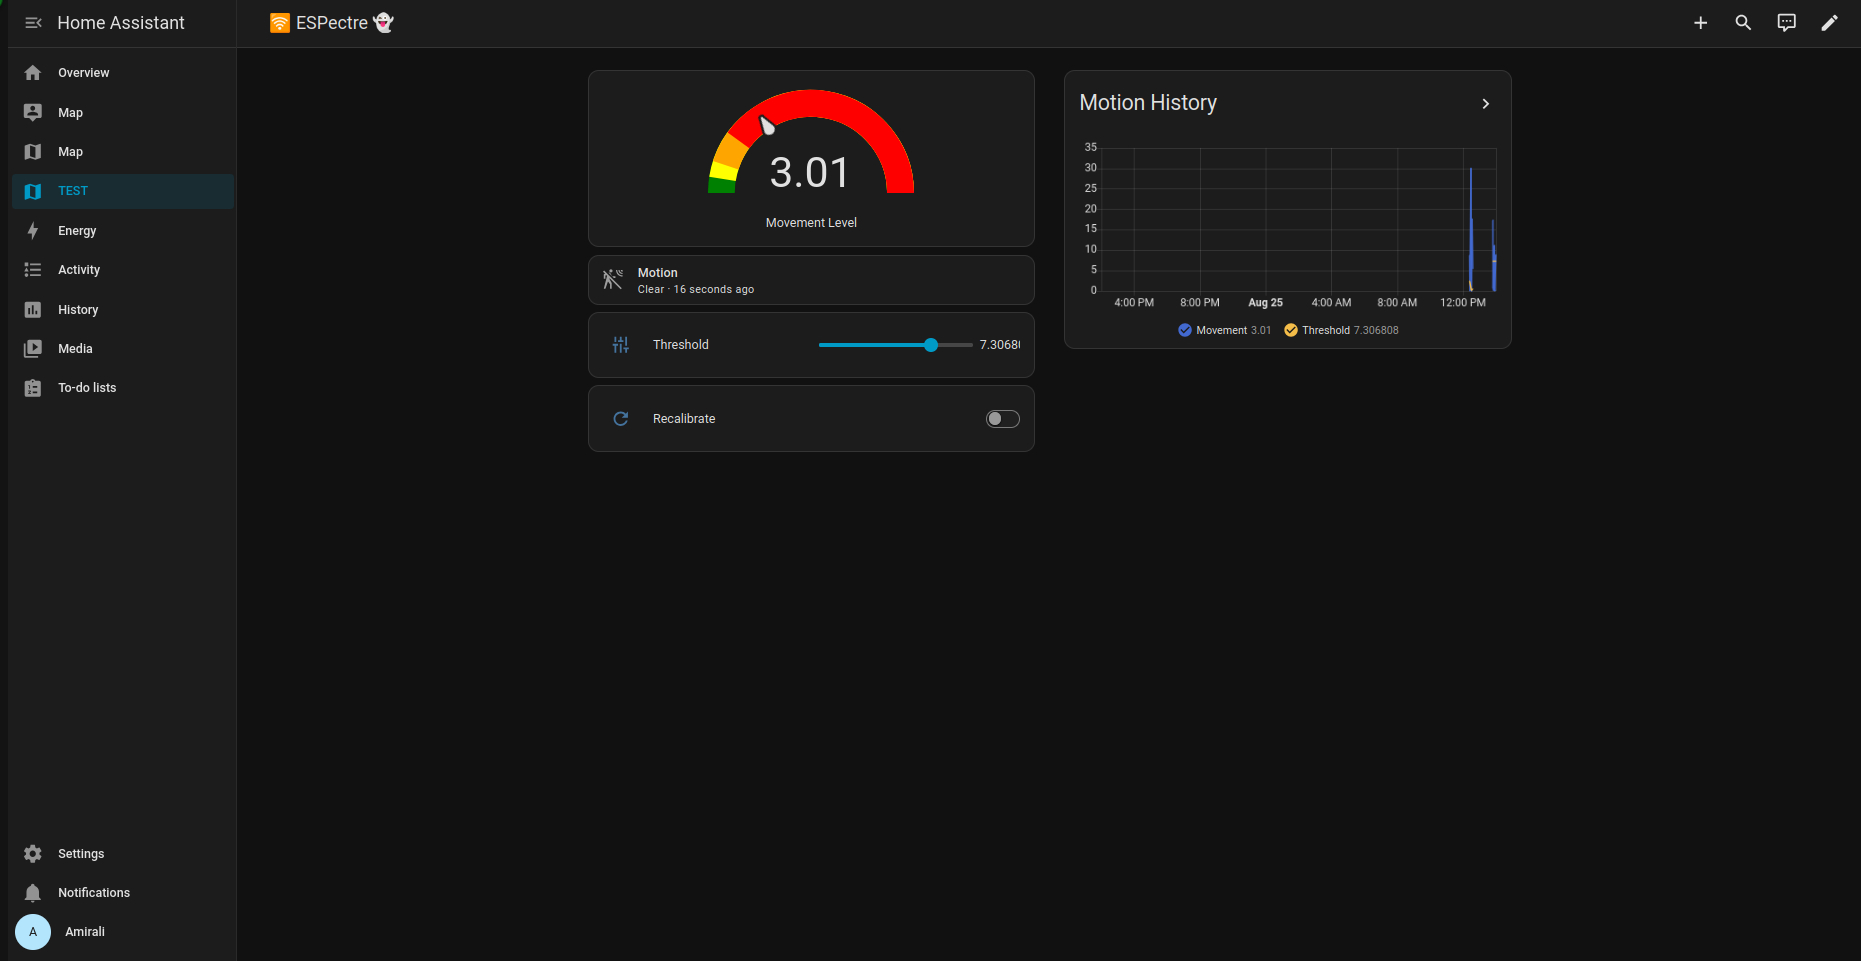
\includegraphics[width=0.85\textwidth]{ImagesPhase3/ph.png}
    \caption{داشبورد نهایی پایش اطلاعات حسگری وای‌فای در \lr{Home Assistant}}
    \label{fig:ha_dashboard}
\end{figure}

\section{نتیجه‌گیری}
در این پروژه، سیستم حسگری \lr{ESPectre} با موفقیت بر روی برد \lr{ESP32-S3} کامپایل و پایدارسازی گردید. با غلبه بر چالش‌های لایه فیزیکی پورت سریال، تنظیم دسترسی‌های کانتینر داکر و تطبیق فرکانس رادیویی، ارتباط بی‌درنگ با \lr{Home Assistant} برقرار شد و قابلیت‌های الگوریتم‌های \lr{MVS} و \lr{ML} در سنجش تلاطم فضایی امواج وای‌فای تثبیت گردید.

\end{document}
